\section{Linear spectroscopy}
\label{sec:linear}

\subsection{Choose a linear model}

Linear spectrum functions take the system, a one-dimensional angular-frequency
axis and the convergence parameter \texttt{eta}. Pulse-dependent functions
also take a \texttt{GaussianPulse}. Each returns a complex array with one
entry per frequency.


The positive parameter \texttt{eta}, in inverse time units, ensures
convergence of the causal frequency transform. For a stable field-free
Liouvillian,
\[
G_\eta(\omega)=\int_0^\infty
 e^{(i\omega-\eta)t}e^{\mathcal L t}\,dt
 =[(\eta-i\omega)I-\mathcal L]^{-1}.
\]
The factor $e^{-\eta t}$ makes the integral decay, but also adds broadening
beyond the physical relaxation and dephasing in the collapse operators.
When using \texttt{eta} only for convergence, choose a small positive value
that does not materially change the spectral features and still permits
stable linear solves. Reduce it and refine the frequency grid together;
compare unnormalized complex responses, including widths and amplitudes.
The tutorial value $\eta=0.02$ is illustrative, not a universal optimum.

\begin{description}
\item[\texttt{finite\_pulse\_linear\_spectrum}]
Gaussian pulse dressing with the full molecular interaction.
\item[\texttt{impulsive\_linear\_spectrum}]
Full molecular interaction in the impulsive limit, without a pulse envelope.
\item[\texttt{short\_pulse\_linear\_rwa\_spectrum}]
RWA molecular response weighted by the Gaussian pulse spectrum.
\item[\texttt{impulsive\_linear\_rwa\_spectrum}]
RWA molecular response in the impulsive limit, without a pulse envelope.
\end{description}
There is no finite-pulse linear RWA function in this version. The four
available functions have these calling patterns:

\par\noindent
\begin{minipage}{\linewidth}
\begin{lstlisting}[style=python]
finite_pulse_linear_spectrum(
    system, pulse, omega, eta, sign=1, rho0=None)
impulsive_linear_spectrum(system, omega, eta, rho0=None)
short_pulse_linear_rwa_spectrum(
    system, pulse, omega, eta, sign=1, rho0=None)
impulsive_linear_rwa_spectrum(
    system, omega, eta, sign=1, rho0=None)
\end{lstlisting}
\end{minipage}\par
The RWA calls need the two dipole components supplied in the first example.
Use \texttt{sign=1} for the positive-frequency field component.

\subsection{Compare the four models}

Continue in the same Python session as the first example, where
\texttt{system} and \texttt{rho\_ss} have been defined. The code below creates
\emph{one figure with two panels}: the real part on the left and the imaginary
part on the right. Both panels contain all four models.

For this comparison the Gaussian prefactor is set to one at zero phase.
Each complex curve is then divided by its own maximum magnitude so that the
figure compares shapes. These separately normalized curves do not compare
absolute amplitudes. The plotting helper uses \texttt{normalize=False}
to retain this common scale for both components. Its optional
\texttt{normalize=True} instead scales the selected real, imaginary or
absolute-value component by that component's own maximum absolute value.

\par\noindent
\begin{minipage}{\linewidth}
\begin{lstlisting}[style=python]
omega = np.linspace(0.5, 1.7, 241)
sigma = 1.25
pulse = pulsus.GaussianPulse(
    omega_L=1.10, sigma=sigma,
    E0=2 / (np.sqrt(2 * np.pi) * sigma),
)
shared = dict(system=system, omega=omega, eta=0.02,
              rho0=rho_ss)
spectra = {
    "Finite pulse, full": pulsus.finite_pulse_linear_spectrum(
        pulse=pulse, sign=1, **shared),
    "Impulsive, full": pulsus.impulsive_linear_spectrum(**shared),
    "Short pulse, RWA": pulsus.short_pulse_linear_rwa_spectrum(
        pulse=pulse, sign=1, **shared),
    "Impulsive, RWA": pulsus.impulsive_linear_rwa_spectrum(
        sign=1, **shared),
}
fig, axes = plt.subplots(1, 2, figsize=(10, 3.8),
                         constrained_layout=True)
styles = ["-", "--", "-.", ":"]
for (name, spectrum), style in zip(spectra.items(), styles):
    scale = np.max(np.abs(spectrum))
    y = spectrum / scale if scale else spectrum
    for ax, component in zip(axes, ["real", "imag"]):
        pulsus.plot_linear_spectrum(
            omega, y, component=component, normalize=False,
            ax=ax, label=name, linestyle=style, linewidth=1.1,
        )
for ax, component in zip(axes, ["Real", "Imaginary"]):
    ax.set_xlabel("Angular frequency (inverse model time)")
    ax.set_ylabel(component + " response / max |complex response|")
    ax.set_title(component + " part: all four models")
    ax.axhline(0, color="0.7", lw=0.6)
    ax.legend(fontsize=7)
plt.show()
\end{lstlisting}
\end{minipage}\par

\begin{figure}[!htbp]
\centering
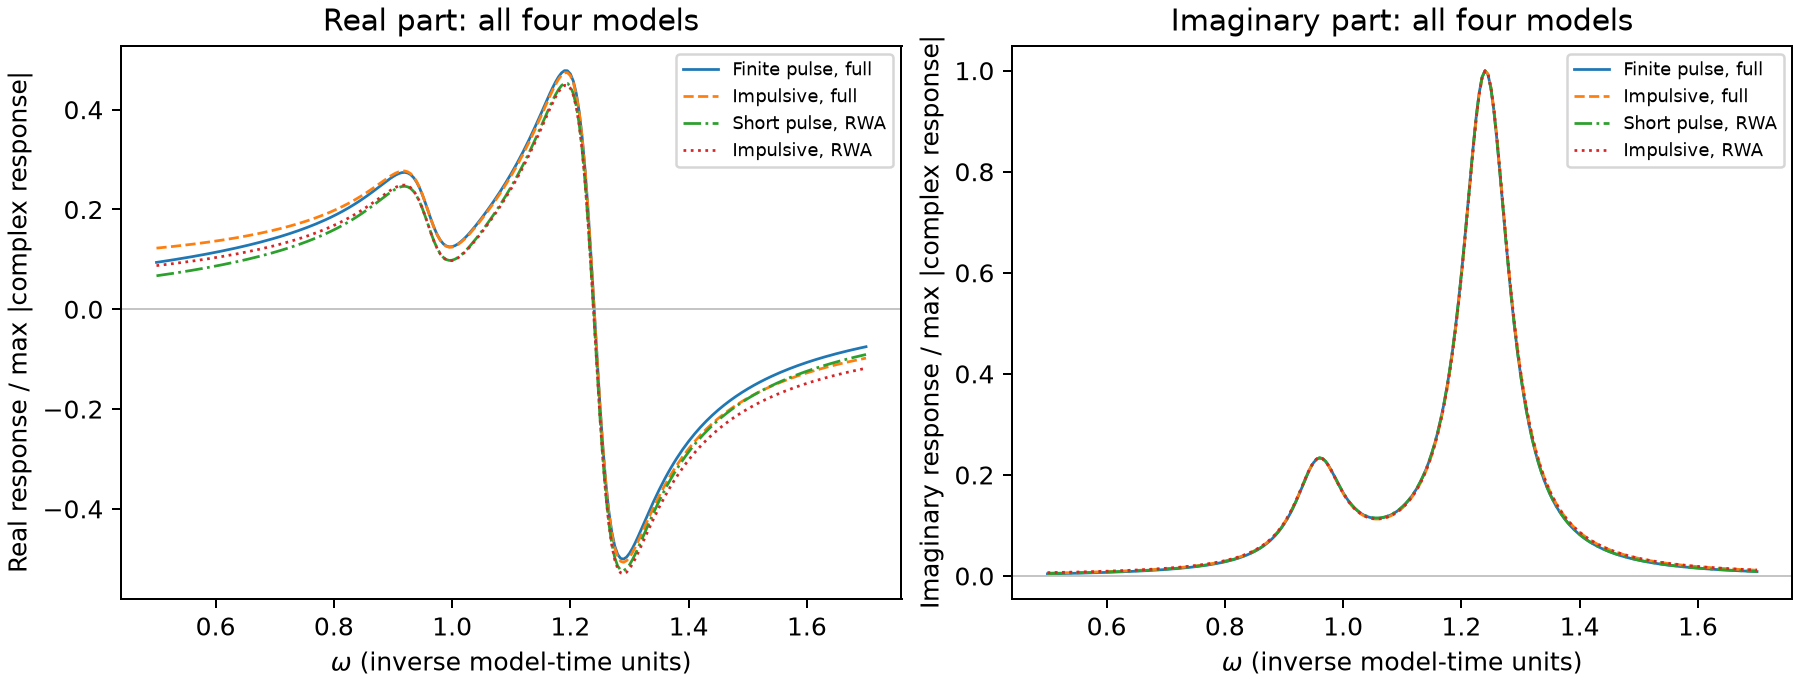
\includegraphics[width=\linewidth]{figures/linear_models.png}
\caption{Real (left) and imaginary (right) parts of the four linear models.
All four curves are present in each panel. For these parameters their
imaginary parts nearly overlap. Distinct line styles are used without markers.
Each complex curve is normalized separately before plotting.}
\label{fig:linear-models}
\end{figure}

\par\noindent
\begin{minipage}{\linewidth}
The script \path{examples/manual/02_linear_models.py} performs this complete
comparison if you have the repository examples. Package-only users can run
the code above after the first example.
\end{minipage}\par

\subsection{Plot and customize a spectrum}

For one curve, the new helper creates a figure when no \texttt{ax} is supplied:
\begin{lstlisting}[style=python]
fig, ax, line = pulsus.plot_linear_spectrum(
    omega, spectra["Finite pulse, full"],
    component="imag", normalize=True,
)
plt.show()
\end{lstlisting}
The default is a line without markers. The helper returns the Matplotlib
figure, axes and line, so labels, colors and other details remain editable.
It neither calls \texttt{plt.show()} nor saves a file by default.
Section~\ref{sec:plot-export} explains optional PNG/PDF export for both
linear and two-dimensional plots.

The calculated spectrum is complex. Use \texttt{S.real}, \texttt{S.imag}, or
\texttt{np.abs(S)} depending on the component you want to inspect. The
functions do not automatically produce a phased absorption coefficient.
Finite-pulse functions include the pulse amplitude and phase; impulsive
functions return the molecular response without these pulse factors.
Record the chosen field scaling when comparing amplitudes across models.

In the finite-pulse full-interaction function, \texttt{sign} selects the
field-frequency component while retaining the complete molecular
interaction. In an RWA function, it also selects the corresponding dipole
interaction. These are distinct choices.
